\documentclass{estilo}
\usepackage[spanish]{babel}
\usepackage{graphicx}
\usepackage{float}
\usepackage{amsmath}        % para los vectores columnas
\usepackage{amsfonts}       % para las negrita de pizarra
\usepackage{amssymb}        % para simbolos matematicos
\usepackage{hyperref}       % para utilizar referencias
\usepackage{multirow}       % para las tablas
\usepackage{dsfont}
\usepackage{listings}
\usepackage{xcolor}
\usepackage{graphicx} 
\definecolor{codegreen}{rgb}{0,0.6,0}
\definecolor{codegray}{rgb}{0.5,0.5,0.5}
\definecolor{codepurple}{rgb}{0.58,0,0.82}
\definecolor{backcolour}{rgb}{0.95,0.95,0.92}
\lstdefinestyle{mystyle}{
    backgroundcolor=\color{backcolour},   
    commentstyle=\color{codegreen},
    keywordstyle=\color{magenta},
    numberstyle=\tiny\color{codegray},
    stringstyle=\color{codepurple},
    basicstyle=\ttfamily\footnotesize,
    breakatwhitespace=false,         
    breaklines=true,                 
    captionpos=b,                    
    keepspaces=true,                 
    numbers=left,                    
    numbersep=5pt,                  
    showspaces=false,                
    showstringspaces=false,
    showtabs=false,                  
    tabsize=2
}
\lstset{style=mystyle}

\usepackage{enumitem,multicol,setspace}
\newcounter{subenum}[enumi] % para las multicolumnas
\renewcommand{\thesubenum}{\arabic{subenum}}
\usepackage[nomessages]{fp}
\FPeval\thecolwidth{round(1/4:4)}% Specify number of columns -> column width
\newcommand{\newitem}[1]{%
  \refstepcounter{subenum}%
  \parbox{\dimexpr\thecolwidth\linewidth-.5\columnsep}{%
    \makebox[\labelwidth][r]{(\thesubenum)\hspace*{\labelsep}}%
    #1}\hfill%
}

\usepackage{scalerel,stackengine} % para el sombrero
\stackMath
\newcommand\rhat[1]{%
\savestack{\tmpbox}{\stretchto{%
  \scaleto{%
    \scalerel*[\widthof{\ensuremath{#1}}]{\kern-.6pt\bigwedge\kern-.6pt}%
    {\rule[-\textheight/2]{1ex}{\textheight}}%WIDTH-LIMITED BIG WEDGE
  }{\textheight}% 
}{0.5ex}}%
\stackon[1pt]{#1}{\tmpbox}%
}
\parskip 1ex

\usepackage{mathtools}      % floor y ceil
\DeclarePairedDelimiter\ceil{\lceil}{\rceil}
\DeclarePairedDelimiter\floor{\lfloor}{\rfloor} 

\usepackage[style=authoryear-comp]{biblatex}


\begin{document}
\maketitle

\justifying{}

%Tabla de contenidos
\newpage
\tableofcontents % Índice general
\newpage

\newpage
\section*{Consigna}


{\Large Introducción}
\vskip0.5cm

Seguimos con la misma situación planteada en el trabajo práctico anterior, pero ahora pasaron varios años. Mateo ahora tiene 7 años. Los mismos años que tenía Sophia cuando comenzaron a jugar al juego de las monedas. Eso quiere decir que Mateo también ya aprendió sobre algoritmos greedy, y lo comenzó a aplicar. Esto hace que ahora quién gane dependa más de quién comience y un tanto de suerte.

Esto no le gusta nada a Sophia. Ella quiere estar segura de ganar siempre. Lo bueno es que ella comenzó a aprender sobre programación dinámica. Ahora va a aplicar esta nueva técnica para asegurarse ganar siempre que pueda.

\vskip0.5cm
{\Large Consigna}
\vskip0.5cm

\begin{enumerate}
    \item Hacer un análisis del problema, plantear la ecuación de recurrencia correspondiente y proponer un algoritmo por programación dinámica que obtenga la solución óptima al problema planteado: Dada la secuencia de monedas m1,m2 .... mn,sabiendo que Sophia empieza el juego y que Mateo siempre elegirá la moneda más grande para sí entre la primera y la última moneda en sus respectivos turnos, definir qué monedas debe elegir Sophia para asegurarse obtener el máximo valor acumulado posible. Esto no necesariamente le asegurará a Sophia ganar, ya que puede ser que esto no sea obtenible, dado por cómo juega Mateo. Por ejemplo, para [1, 10, 5] , no importa lo que haga Sophia, Mateo ganará.
    \vskip0.3cm
    \item Demostrar que la ecuación de recurrencia planteada en el punto anterior en efecto nos lleva a obtener el máximo valor acumulado posible.
    \vskip0.3cm
    \item Escribir el algoritmo planteado. Describir y justificar la complejidad de dicho algoritmo. Analizar si (y cómo) afecta a los tiempos del algoritmo planteado la variabilidad de los valores de las monedas.
    \vskip0.3cm
    \item Realizar ejemplos de ejecución para encontrar soluciones y corroborar lo encontrado. Adicionalmente, el curso proveerá con algunos casos particulares que deben cumplirse su optimalidad también.
    \vskip0.3cm
    \item Hacer mediciones de tiempos para corroborar la complejidad teórica indicada. Agregar los casos de prueba necesarios para dicha corroboración (generando sus propios sets de datos). Esta corroboración empírica debe realizarse confeccionando gráficos correspondientes, y utilizando la técnica de cuadrados mínimos. Para esto, proveemos una explicación detallada, en conjunto de ejemplos.
    \vskip0.3cm
    \item Agregar cualquier conclusión que les parezca relevante.
\end{enumerate}



\newpage

\justifying{
\hypertarget{res}{\section*{Resolución}}
\section{Ecuación de recurrencia}

A continuación se mostrará la \textbf{ecuación de recurrencia} hallada para este
problema:

\vskip0.5cm

\begin{center}
  
    $T(monedas, inicioFila, finFila) = \left\{ \begin{array}{lcc} K_{1} & si & K_{1} > K_{2} \\ \\ K_{2} & si & K_{1} < K_{2} \\  \end{array} \right.$

\end{center}

Siendo 

\vskip0.25cm

\begin{center}
  
    $K_{1} = monedas[inicioFila] + T(monedas, S(monedas, inicioFila + 1, finFila))$

    \vskip0.1cm
    $K_{2} = monedas[finFila] + T(monedas, S(monedas, inicioFila, finFila - 1))$
\end{center}


donde


$S(monedas, inicioFila, finFila) = \left\{ \begin{array}{lcc} (inicioFila+1,finFila) & si & monedas[inicioFila] > monedas[finFila] \\ \\ (inicioFila, finFila - 1) & si &  monedas[inicioFila] < monedas[finFila] \\  \end{array} \right.$

\vskip0.5cm

\textbf{NOTA}: 

$monedas$ = El vector con los valores de las monedas

$inicioFila$ = Es el valor de la primera moneda del vector monedas

$finFila$ = Es el valor de la última moneda del vector monedas

\vskip0.5cm

Nuestra función $T(monedas, inicioFila, finFila)$ nos otorga la ganancia que consiguió Sophia al momento de jugar con una cantidad de $n$ monedas contra Mateo. En esta, podemos observar como nuestras variables $K_{1}$ y $K_{2}$
realizan llamados recursivos a $T$ teniendo en cuenta como variables $inicioFila$ y $finFila$ la salida de otra función llamada $S(monedas, inicioFila, finFila)$ , que son las dos posibles decisiones que puede tomar mateo al elegir una moneda (recordemos que mateo sigue las reglas del juego estríctamente).
\section{Demostración: NP-Completo}


\subsection*{Reducción desde el problema 3-Partition en su version unaria}

Vamos a demostrar que la batalla naval es $NP$-Completo. Pero, ¿Como se demuestra que un problema es $NP$-Completo? Tiene que cumplir dos condiciones: 

\begin{itemize}
    \item \textbf{Pertenencia a NP:} La verificación de una solución candidata es posible en tiempo polinomial.
    \item \textbf{NP-dificultad:} Se puede realizar una reducción polinomial desde cualquier problema NP-completo hacia este problema.
\end{itemize}

Ya en la sección anterior pudimos verificar con éxito que nuestro problema es un problema NP, ahora hay que demostrar que se puede realizar una reducción polinomial desde cualquier problema NP-Completo. Recordemos que todos los NP completos pueden ser reducidos despues cualquier problema NP completo. 

En nuestro caso, utilizaremos el problema de \textit{3-Partition}, que como demostraremos más abajo, es un problema NP-Completo, para verificar que el problema de la batalla naval pertenece a NP-Completo. Es decir, se puede realizar la reduccion polinomial: \textbf{3-Partition} $\leq_p$ \textbf{PBN}.

Definamos un poco cómo se compone el problema \textit{3-Partition}.

\textbf{Nota}: Por simplificacion, siempre que hablemos de 3-Partition, nos estamos refiriendo a la version unaria del problema.

\subsubsection*{Definición del problema 3-Partition}

Dado un conjunto de enteros positivos \(S = \{a_1, a_2, \dots, a_{n}\}\), donde cada número está representado en notación unaria, decide si el conjunto puede partirse en 3 subconjuntos disjuntos \(S_1, S_2, S_3\), tal que la suma de cada subconjunto sea la misma. Es decir:

\begin{itemize}
    \item La suma de los elementos de cada subconjunto \(S_i\) = m
    \item sum(S) = \(sum(S_1) + sum(S_2) + sum(S_3)\) = 3m
\end{itemize}

Veamos un ejemplo: 

$S = \{1, 111, 11, 1, 1, 1\}$

\textbf{Nota}: Es la representacion unaria de $S = \{1, 3, 2, 1, 1, 1\}$

Una solución a esta instancia del problema de 3-Partition es la siguiente:

$S_1 = \{111\}$, $S_2 = \{11, 1\}$, $S_3 = \{1, 1, 1\}$

Vemos que es solución, ya que se cumple que la suma de los elementos en cada subconjunto $S_i = 3$. %Y los subconjuntos S_i son disjuntos.%

\section*{Reducción de 2-Partition a 3-Partition}

\subsection*{Definiciones}

\textbf{2-Partition:} El problema consiste en dividir un conjunto de números \( A = \{a_1, a_2, \dots, a_n\} \) en dos subconjuntos disjuntos \( S_1 \) y \( S_2 \) tales que la suma de los elementos de ambos subconjuntos sea igual.

\textbf{3-Partition:} El problema consiste en dividir un conjunto de números (en representacion unaria) \( B = \{b_1, b_2, \dots, b_n\} \) en tres subconjuntos disjuntos \( S_1, S_2, S_3 \), tales que la suma de los elementos en cada subconjunto sea la misma.

\subsection*{Pertenencia a NP}

Primero hay que demostrar que 3-Partition pertenece a NP, para ello, debemos poder encontrar un validador que valide una solución al problema de 3-Partition en tiempo polinomial. Dicho validador es el siguiente:

Dado \( S = \{a_1, a_2, \dots, a_n\} \), y tres subconjuntos $S_1$, $S_2$, y $S_3$, se valida que:

\begin{itemize}
    \item $S$, $S_1$, $S_2$, $S_3$ estan en representacion unaria (lo estan si su representacion consiste en $a_i$ veces el numero 1)
    \item $sum(S_1)$ = $sum(S_2)$ = $sum(S_3)$
    \item $S_1$ $\cup$ $S_2$ $\cup$ $S_3$ = $S$
    \item $S_1$ $\cap$ $S_2$ $\cap$ $S_3$ = $\emptyset$
\end{itemize}

Dado que verificar la representacion unaria, comprobar que los subconjuntos son disjuntos, calcular la suma de los elementos de cada subconjunto, verificar que la sumas de cada subconjunto son iguales, se puede hacer en tiempo polinomial, decimos que 3-Partition esta en NP.

\subsection*{Reducción}

Para reducir polinomialmente una instancia de \textbf{2-Partition} a una instancia de \textbf{3-Partition}, hacemos lo siguiente:

Consideramos el conjunto \( S = \{a_1, a_2, \dots, a_n\} \) tal que $sum(S) = 2m$. Donde $m = sum(S_1) = sum(S_2)$.

Lo que debemos hacer, es calcular m, y agregarlo al conjunto S. Luego, realizamos la representacion unaria de los elementos de S, y resolvemos el problema usando la caja negra de 3-Partition. Si hay solución para 3-Partion, hay solución para 2-Partition.

Veamoslo con un ejemplo:

$S = \{3, 4, 3, 4\}$. Una solución al problema de 2-Partition es la siguiente: $S_1 = \{3, 4\}$, $S_2 = \{3, 4\}$. Pero vamos a resolverlo usando 3-Partition de la forma que mencionamos arriba, es decir, vamos a transformar esta instancia a una que pueda resolverse con 3-Partition.

Vemos que $m = sum(S)$ $/$ $2 = (3 + 4 + 3 + 4)$ $/$ $2 = 7$, entonces al agregar a $m$ al conjunto $S$ y representar todo de forma unaria, tenemos $S = \{111, 1111, 111, 1111, 1111111\}$. Y usando la caja negra de 3-Partition, vemos que hay solución. De hecho, es la siguiente:

$S_1 = \{111, 1111\}$, $S_2 = \{111, 1111\}$, $S_3 = \{1111111\}$.

\textbf{Nota}: Siempre vamos a encontrar que un tercer subconjunto va a ser exactamente m, y por lo tanto, sumar exactamente m tambien (que es lo que por supuesto, suman los otros 2 subconjuntos).

Si pudimos encontrar estos 3 subconjuntos, implica que hay solución para 2-Partition, ya que ahora en 3-Partition $sum(S) = 3m = 2m + m$, y esto solo sucede si $sum(S_1) = sum(S_2) = sum(S_3) = m$, que significa que en la instancia original de 2-Partition existe solución tal que $sum(S) = 2m$, siendo $sum(S_1) = m$, $sum(S_2) = m$.

% FALTA DEMOSTRAR CORRECTAMENTE QUE ESTO ES COMPLEJIDAD POLINOMIAL %
Dado que encontrar m, agregar m al conjunto S y representar a los elementos de S en forma unaria, pueden hacerse en tiempo polinomial. Entonces pudimos hacer la reduccion \textbf{2-Partition} $\leq_p$ \textbf{3-Partition}. Quedando demostrado que 3-Partition pertenece a NP-Completo.

% DE ACA PARA ABAJO LA MAYOR PARTE ESTA MAL (HAY QUE REHACER VARIAS COSAS USANDO LA VERSION UNARIA DE LA VARIACION DEL 3-PARTITION)

\subsection*{Reducción de 3-Partition a La Batalla Naval}


Dado una instancia del problema \textit{3-Partition}, construiremos una instancia del problema \textit{La Batalla Naval}.

\paragraph{Construcción del tablero:}

\begin{itemize}
    \item \textbf{Dimensiones del tablero:} % IMPORTANTE: Quiza invirtiendo la logica entre filas/columnas sea mas facil o igual %
    \begin{itemize}
        \item Cantidad de filas: 5. Cada subconjunto \(S_i\) ocupa una fila, y se agrega una fila vacía después de cada subconjunto (excepto después del último).
        \item Cantidad de columnas: $sum(S)$ = \(3m\). % NO ESTOY SEGURO %
    \end{itemize}

    \item \textbf{Restricciones de las filas:}
    \begin{itemize}
        \item Las filas que contienen subconjuntos tienen una restricción igual a $m$.
        \item Las filas vacías (entre subconjuntos) tienen una restricción igual a 0.
    \end{itemize}

    \item \textbf{Restricciones de las columnas:} Las restricciones de las columnas van a ser 1 para todas. Ya que en cada columna va a haber exactamente una parte de un barco.

    \item \textbf{Barcos:} Los barcos van a ser los elementos $a_i$ que pertenecen al conjunto S.
\end{itemize}

% ME QUEDE ACA


\section*{Ejemplos}

A continuación desarrollaremos 2 ejemplos para visualizar la relación entre 3-Partition y la Batalla Naval:

\textbf{Instancia del problema de 3-Partition:}
\[
S = \{1, 111, 11, 1, 1, 1\}
\]

\textbf{Pasamos a no unario:}
\[
S = \{1, 3, 2, 1, 1, 1\}
\]

\textbf{Calculamos la suma total y hallamos m:}
\[
\text{sum}(S) = 9 = 3m \rightarrow m = 3
\]

\textbf{Lo transformamos a un problema de batalla naval:}

\[
\text{Filas} = [3, 0, 3, 0, 3]
\]
\[
\text{Columnas} = [1, 1, 1, 1, 1, 1, 1, 1, 1]
\]
\[
\text{Barcos} = [1, 3, 2, 1, 1, 1]
\]

\textbf{Usamos la caja negra de la batalla naval. Veamos una posible solución:}
\[
\begin{array}{ccccccccc}
1 & 1 & 1 & - & - & - & - & - & - \\
- & - & - & - & - & - & - & - & - \\
- & - & - & 1 & - & - & 1 & - & 1 \\
- & - & - & - & - & - & - & - & - \\
- & - & - & - & 1 & 1 & - & 1 & - \\
\end{array}
\]

Vemos que se cumplen las restricciones de las filas, ya que la primer, tercera y quinta fila tienen 3 de demanda cumplida en cada una.
También se cumplen las restricciones de las columnas, pues en cada una de ellas se coloca exactamente una parte de un barco.
Además vemos que se están colocando todos los barcos (los 6 barcos), respetando las restricciones de adyacencia.
Por lo tanto, dada esta configuración de demandas de filas, columnas y longitudes de barcos, vemos que existe una solución al problema de la batalla naval.

% \noindent\rule{\textwidth}{0.5pt}

\subsection{Veamos otro ejemplo:}

\textbf{Instancia del problema de 3-Partition:}
\[
S = \{111111, 11111, 1111, 11111, 111, 1111111\}
\]

\textbf{Pasamos a no unario:}
\[
S = \{6, 5, 4, 5, 3, 7\}
\]

\textbf{Calculamos la suma total y hallamos m:}
\[
\text{sum}(S) = 30 = 3m \rightarrow m = 10
\]

\textbf{Nota:} Solución válida de 3-partition:
\[
    \{1111111, 111\}, \{111111, 1111\}, \{11111, 11111\}
\]

\textbf{Lo transformamos a un problema de la batalla naval:}

\[
\text{Filas} = [10, 0, 10, 0, 10]
\]
\[
\text{Columnas} = [1, 1, 1, 1, 1, 1, 1, 1, 1, 1, 1, 1, 1, 1, 1, 1, 1, 1, 1, 1, 1, 1, 1, 1, 1, 1, 1, 1, 1, 1]
\]
\[
\text{Barcos} = [6, 5, 4, 5, 3, 7]
\]

\textbf{Usamos la caja negra de la batalla naval. Veamos una posible solución:}
\[
\scriptsize
\begin{array}{cccccccccccccccccccccccccccccc}
1 & 1 & 1 & 1 & 1 & 1 & 1 & - & - & - & - & - & - & - & - & - & - & - & 1 & 1 & 1 & - & - & - & - & - & - & - & - & - \\
- & - & - & - & - & - & - & - & - & - & - & - & - & - & - & - & - & - & - & - & - & - & - & - & - & - & - & - & - & - \\
- & - & - & - & - & - & - & 1 & 1 & 1 & 1 & 1 & 1 & - & - & - & - & - & - & - & - & 1 & 1 & 1 & 1 & - & - & - & - & - \\
- & - & - & - & - & - & - & - & - & - & - & - & - & - & - & - & - & - & - & - & - & - & - & - & - & - & - & - & - & - \\
- & - & - & - & - & - & - & - & - & - & - & - & - & 1 & 1 & 1 & 1 & 1 & - & - & - & - & - & - & - & 1 & 1 & 1 & 1 & 1 \\
\end{array}
\]

Al igual que en el ejemplo anterior, vemos que se cumplen las restricciones de las filas, pues la primer, tercera y quinta fila tienen 10 de demanda cumplida cada una.
También se cumplen las restricciones de las columnas, pues en cada columna se coloca exactamente una parte de un barco.
Además vemos que se estan colocando todos los barcos (los 6 barcos), respetando las restricciones de adyacencia.
Por lo tanto, dada esta configuración de demandas de filas, columnas y longitudes de barcos, vemos que existe una solución al problema de la batalla naval.

\paragraph{Relación con 3-Partition:}
\begin{itemize}
    \item Cada subconjunto \(S_i\) corresponde a una fila del tablero. 
    \item Los elementos de cada subconjunto \(S_i\) son equivalentes a los barcos en la batalla naval, ocupando exactamente \(m\) celdas en esa fila.
    \item Si se puede resolver el problema de la batalla naval, tras configurar el tablero cumpliendo todas las restricciones mencionadas anteriormente, entonces existe una solución para el problema de \(3\)-Partition.
\end{itemize}

\subsection{Hay 3-Partition $\rightarrow$ hay PBN:}

Supongamos que hay solución en 3-Partition, es decir, dado un conjunto $S$ en representación unaria, pudimos
encontrar $S_1$, $S_2$, $S_3$ subconjuntos disjuntos de $S$ tal que $sum(S1)$ = $sum(S2)$ = $sum(S3)$ = $m$.

Resulta entonces: 

\begin{itemize}
    \item Los elementos de cada subconjunto $S_i$ van a estar en una fila de la matriz en la solución de nuestro problema de la batalla naval.
    \item Los barcos van a ser representados por los elementos de $S_i$, tal que su longitud van a ser igual al valor de dicho elemento.
    \item La cantidad de filas van a ser 5. Para respetar las restricciones sobre la adyacencia, hay que colocar una fila vacía tras colocar cada una de las filas que representan los subconjuntos, salvo la última. Luego la demanda de las filas que representan los subconjuntos va a ser igual a $m$, y las filas vacías van a tener de demanda 0.
    \item La cantidad de columnas van a ser $sum(S)$, y van a tener todas restricción 1, para asegurarnos de que en una misma columna solo se va a colocar una parte de un barco.
\end{itemize}
Como pudimos encontrar 3 subconjuntos del conjunto $S$ que cumplen con las características del problema 3-Partition, resulta que, siempre vamos a poder encontrar una configuración válida para la batalla naval, en la cual cada subconjunto $S_i$ representa una fila y $sum(S)$ representa la cantidad de columnas. Además, la demanda cumplida en cada fila con demanda mayor a 0 es igual a $m$, y la demanda cumplida en cada columna es igual a 1.
    
\subsection{Hay PBN $\rightarrow$ hay 3-Partition:}

\begin{itemize}
    \item Tendremos una configuración en donde la tabla se compone de 5 filas, las cuales 3 tienen demanda mayor a 0 y 2 con demanda igual a 0, y $sum(S)$ columnas con demanda igual 1.
    \item Al colocar los barcos en dichas filas, resulta que estas se mapean a un subconjunto del problema de 3-Partition: Al tener 3 filas con demanda mayor a 0, tendremos 3 subconjuntos.
    \item La demanda cumplida es igual en todas las filas cuya demanda es mayor a 0.
\end{itemize}
Como pudimos encontrar una disposición de barcos que cumplan con la demanda pedida, resulta que hay solución en 3-Partition tal que cada fila no vacía va a ser un subconjunto, y los barcos colocados en dicha fila, van a ser los elementos que pertenecen al subconjunto en cuestión.

\subsection*{Conclusión}

\begin{itemize}
    \item \textit{La Batalla Naval} pertenece a NP.
    \item Reducimos un problema NP-completo (\textit{3-Partition}) a \textit{La Batalla Naval} en tiempo polinomial.
    \item Si existe una solución para el problema \textit{3-Partition}, entonces podemos construir una configuración válida del tablero para \textit{La Batalla Naval}.
    \item Si existe una configuración válida para \textit{La Batalla Naval}, entonces podemos construir una partición válida para el problema \textit{3-Partition}.
\end{itemize}

Por lo tanto, \textit{La Batalla Naval} es NP-completo.
\section{Algoritmo de Backtracking}
\label{sec:backtracking}

\subsection{Codigo}

\lstinputlisting[language=python]{code/backtracking.py}

\subsection{Análisis}

Estamos probando todas las combinaciones posibles, al iterar por todos los barcos y por cada uno, iterar por cada casillero de la matriz. En cada posición del casillero, estamos intentando meter el barco, tanto vertical como horizontalmente, y también consideramos el caso de que no se ponga dicho barco. Esto nos termina dando una complejidad exponencial en cantidad de barcos, ya que como mencionamos al principio, estamos probando todas las combinaciones posibles, por lo tanto: O(2$^n$).

Estamos realizando dos podas:

\begin{itemize}
    \item Si el barco por el que estoy iterando no cabe por la capacidad máxima de la fila o la columna (que tenga mayor valor entre ambos máximos), entonces el barco no se puede meter en la solución actual, por lo que se pasa al siguiente barco. 
    \item Sumamos los barcos que nos quedan por colocar (multiplicado por 2), y eso es como mucho lo máximo que puede mejorar nuestra solución. Si no supera la mejor solución ya obtenida, no tiene sentido seguir, por lo que se poda la rama.
\end{itemize}
\section{Ejemplos de ejecución}
Se pueden encontrar encontrar multiples ejemplos de ejecución dentro del directorio \textit{ejemplos} en el repositorio. Veamos algunos:

Supongamos que tenemos 5 monedas:

\begin{lstlisting}
    [96, 594, 437, 674, 950]
\end{lstlisting}

En cada turno, Sophia tiene la opcion de elegir 2 monedas, la del principio o la del final. Esto implica que cada turno puede representarse como 2 opciones posibles, donde se debe elegir la opcion que acumule el mayor valor.

Para esto se recorren las opciones de manera recursiva, y se va seleccionando el maximo de los valores agregados en cada turno.

De esta forma, como se puede observar en el siguiente grafico, Sophia puede obtener un maximo de 1.483 puntos.

\begin{center}
    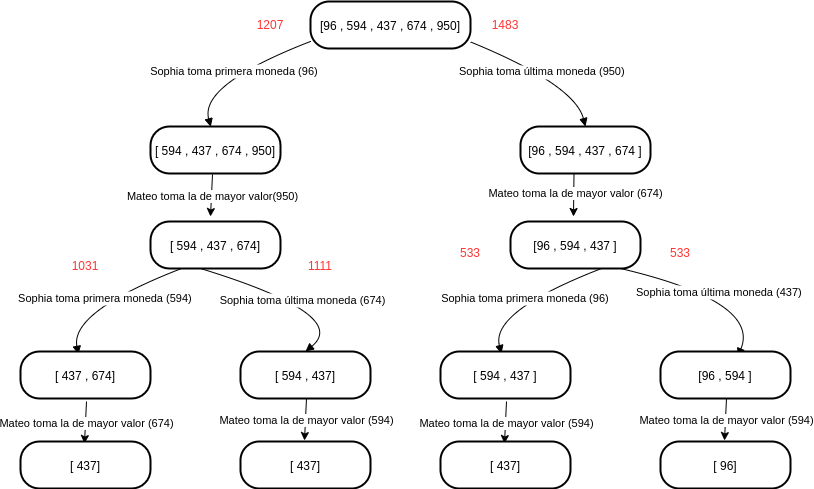
\includegraphics[scale = 0.5]{ {images/TDA-TP2.png} } 
\end{center}

Veamos lo que obtenemos al ejecutar en código el ejemplo que acabamos de ver:

\begin{center}
    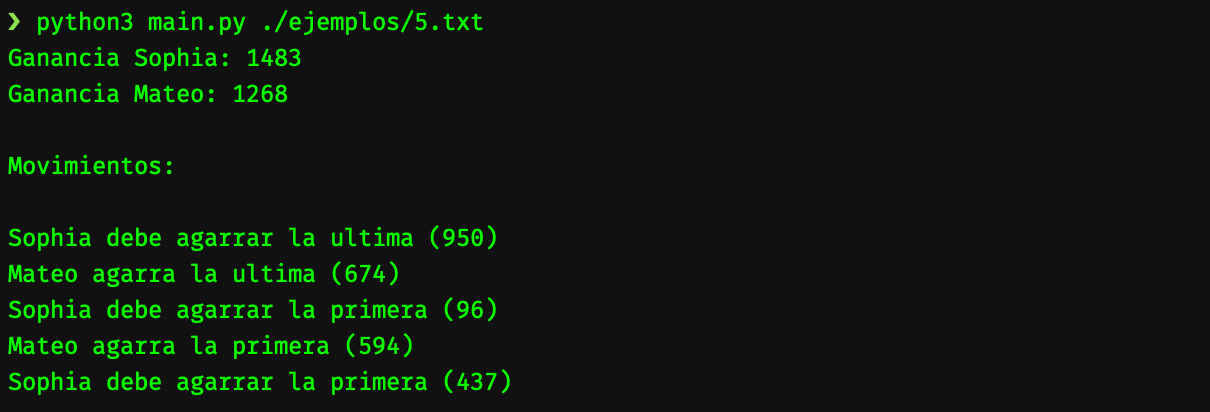
\includegraphics[scale = 0.6]{ {images/screen3.png} } 
\end{center}

Veamos la ejecución de otros ejemplos brindados por la cátedra:
\vskip0.5cm
Este ejemplo es con 10 monedas:
\begin{center}
    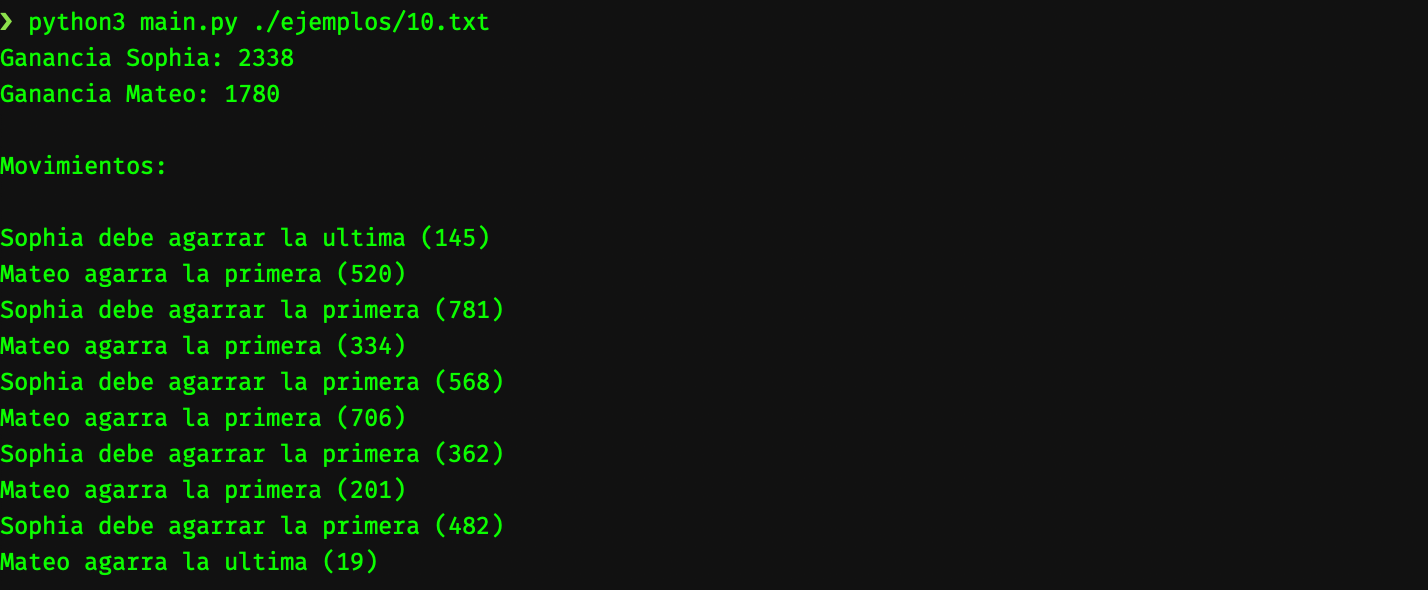
\includegraphics[scale = 0.6]{ {images/screen1.png} } 
\end{center}
Este ejemplo es con 25 monedas:
\begin{center}
    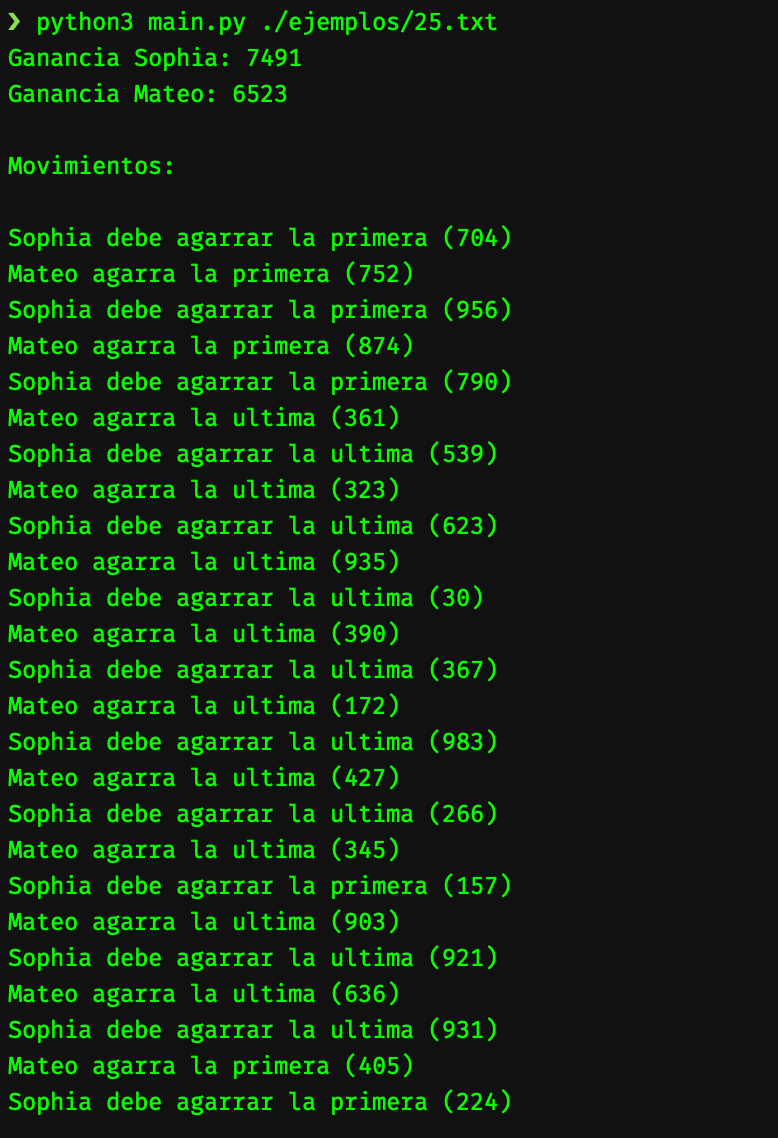
\includegraphics[scale = 0.6]{ {images/screen2.png} } 
\end{center}

Como podemos observar, los resultados obtenidos coinciden con los \textit{Resultados esperados} compartidos por la cátedra.

Ademas de estos ejemplos, se pueden encontrar otros en el directorio \textit{ejemplos} del repositorio. Los mismos pueden ser ejecutados con el comando \textit{pytest -v -s} en la terminal.

\begin{center}
    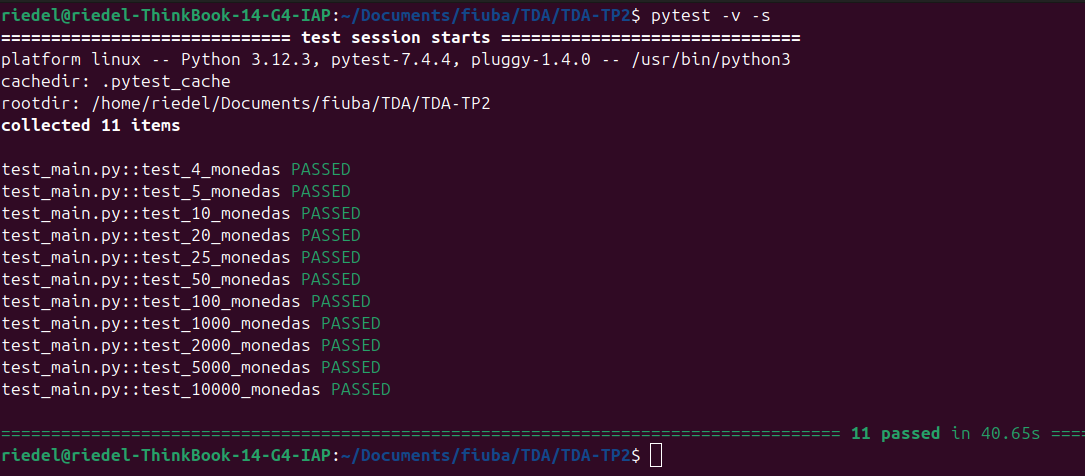
\includegraphics[scale = 0.4]{ {images/tests.png} } 
\end{center}
\section{Algoritmo de aproximación}

\section{Medición empírica}

Para comprobar empíricamente la complejidad \textbf{O($2^n$)} del algoritmo, se decidió ejecutar el mismo con distintos tamaños de entrada y medir el tiempo de ejecución. Se generaron muestras de tamaño $n$, las cuales varían desde $10$ hasta $1000$.

Para cada muestra se registró el tiempo de ejecución, obteniendo el siguiente gráfico:

\begin{center}
    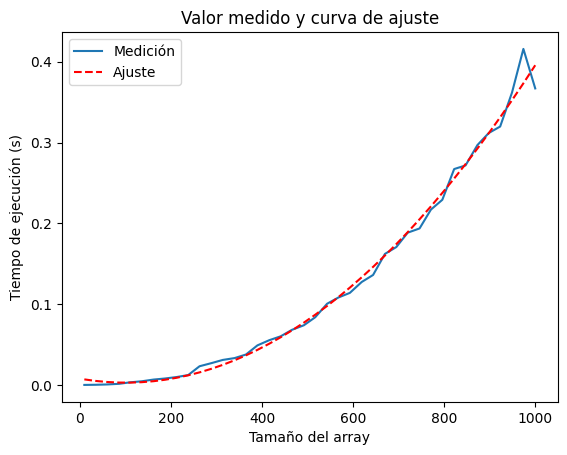
\includegraphics[scale = 0.6]{ {images/cuadradosMinimos.png} }
\end{center}


A simple vista se puede observar un crecimiento $exponencial$. Para confirmar esto, vamos a ajustar los datos a una recta mediante cuadrados mínimos. Esto lo realizamos con \textit{Python} y la función \textit{optimize.curve\_fit} de la biblioteca \textit{scipy}.

Obtenemos que el gráfico se puede ajustar a la curva $y = 1.45e^{-2} \times 2^{x}$, con un error cuadrático medio de $1.485e^{-1}$. Por lo tanto, podemos verificar lo que ya vimos en la sección~\ref{sec:backtracking}, que el orden es exponencial \textbf{O($2^n$)}.

\begin{center}
    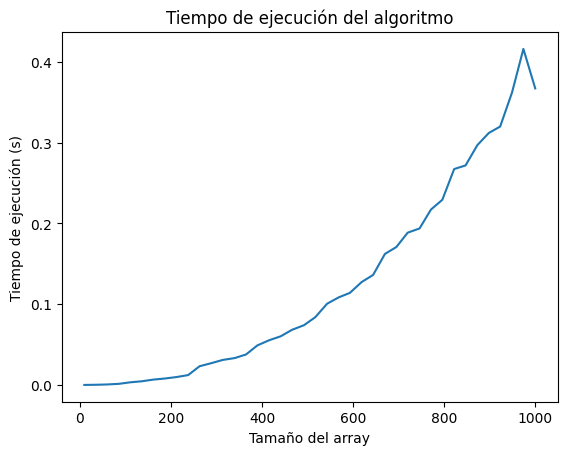
\includegraphics[scale = 0.6]{ {images/image.png} } 
\end{center}
\section{Conclusiones}

En este trabajo práctico, vimos dos versiones del problema de la batalla naval. Por un lado, tenemos un problema NP-Completo, donde intentamos colocar los barcos de forma tal que se cumplan las demandas de todas las filas y columnas, siempre respetando las restricciones de adyacencias. Como demostramos en las secciones anteriores, el problema es de tipo NP y lo pudimos demostrar realizando una reducción polinomial de otro problema NP-Completo como es 3-Partition.

Luego vimos otra variante del problema, en la cual minimizamos la demanda incumplida utilizando un algoritmo de Backtracking.

Por último, implementamos el algoritmo que nos propone John Jellicoe, el cual no nos lleva a la solución óptima, pero nos permite aproximarnos con una cota inferior de $0,3604$, lo cual es aproximádamente un $33\%$ de la solución óptima.

}


\newpage
\end{document}